\documentclass{beamer}
%~ \usetheme{Hannover}  %% Themenwahl
%~ \usetheme{Bergen}  %% Themenwahl
\usetheme{Berkeley}  %% Themenwahl
\usecolortheme{dove}

\usepackage[utf8]{inputenc}
\usepackage[T1]{fontenc}

\usepackage[ngerman]{babel}

\usepackage{graphicx}
\usepackage{upgreek}
\usepackage{float}
\usepackage{units}
\usepackage{url}

\usepackage{subfigure}

\usepackage{amsmath}
\usepackage{amssymb}
\usepackage{amsfonts}

\usepackage{longtable}

\usepackage{ae}
\usepackage{booktabs}

\usepackage{tikz}
\usetikzlibrary{patterns}

%\abs{Ausdruck} %Betragsstriche, die skalieren - abgekürzt
\newcommand{\abs}[1]{\ensuremath{\left\vert#1\right\vert}}
% und das gleiche füur große Klammern
\newcommand{\brac}[1]{\ensuremath{\left(#1\right)}}
% Erwartungswert skalierend
\newcommand{\avg}[1]{\left< #1 \right>}
% ein nicht kursives d für Ableitungen/Integrale, mit etwas Platz davor, um sich etwas abzusetzten
\newcommand{\de}{\ensuremath{\,\mathrm{d}}}
% Für Einheiten: schreibt sie nicht kursiv und lässt etwas Platz zur Zahl vorher
\newcommand{\eh}[1]{\ensuremath{\,\mathrm{#1}}}
% einfaches Gradzeichen
\newcommand{\gr}{\ensuremath{^{\circ}}}
% Fehlerfortpfanzung
% dy/dz * delta z
\newcommand{\fehler}[2]%
{\ensuremath{\abs{\frac{\partial #1}{\partial #2}}\cdot \Delta #2}}

\title{Ising-Ferromagnet auf Ad-Hoc Netzwerken}
\author{Hendrik Schawe}
\date{\today}

\begin{document}

\maketitle
\frame{\tableofcontents[pausesections]}

\section{Modell}
    \subsection{Ising Ferromagnet}
        \begin{frame}{Ising Ferromagnet}
            \begin{itemize}[<+->]
                \item \(N\) Knoten (Gitterplätze)
                \item \(\avg{i,j}\) bezeichnet "nächste Nachbar"\ Beziehung
                \item jeder Knoten hat einen Spin \(s \in \{-1,+1\}\){}
                \item Zwei Spins \(i,j\) sind verbunden über \(J_{ij}\)
                \item{
                    \begin{equation}
                        H = - \sum_{\avg{i,j}}J_{ij}s_{i}s_{j}.
                    \end{equation}
                    (Ref.\ \cite{Ising1925})
                }
            \end{itemize}
        \end{frame}

        \begin{frame}{Ungeordneter Ising Ferromagnet}
            \begin{columns}[t]
                \begin{column}{5cm}
                    \begin{itemize}
                        \item<1-> beginne mit einem Quadratgitter
                        \item<2-> verschiebe jeden Knoten nach der Verteilung\\
                            \(f(x)=\frac{1}{\sqrt{2\pi}\sigma}\mathrm{e}^{-\frac{x^2}{2\sigma^2}}.\){}
                        \item<3-> bestimme neue "nächste Nachbarn"
                        \item<4-> bestimme neue abstandsabhängiges \(J_{ij} = e^{\alpha(1-d_{ij})}\)
                        \item<4-> hier \(\alpha = 0.5\)
                    \end{itemize}
                \end{column}
                \begin{column}{6cm}
                    \visible<2->{
                        \vspace{-1cm}
                        \begin{figure}[htbp]
                            \centering
                            \begin{tikzpicture}[scale=1.5, declare function={
        normal(\x,\m,\y) = 1/exp((\x-\m)*(\x-\m)/2/(\s^2))-\y;
      }]
    \def\s{0.5}

    \draw[dashed] (-2,0) -- (4,0);
    \draw[dashed] (0,-2) -- (0,2);
    \draw[dashed] (2,-2) -- (2,2);

    \def\dxa{0.4}
    \def\dya{-0.8}

    \draw (\dxa,\dya) -- node [below] {$\Delta x$} (0,\dya);
    \draw (\dxa,\dya) -- node [right] {$\Delta y$} (\dxa,0);
    \draw[loosely dotted] (\dxa,0) -- (\dxa,{1.6+normal(\dxa,0,0)});
    \draw[loosely dotted] (0,\dya) -- ({-1.6-normal(\dya,0,0)},\dya);
    \draw[->] (0,0) -- (0+\dxa*0.9,0+\dya*0.9);

    \draw[color=black,domain=-1.5:1.5] plot [smooth] (\x,{normal(\x,0,0)+1.6}) node[right] {};
    \fill (0, 0) circle(0.08);
    \draw[color=black] (0+\dxa, 0+\dya) circle(0.08);
    \draw[color=black,domain=-1.5:1.5,rotate=90] plot [smooth] (\x,{normal(\x,0,0)+1.6}) node[right] {};

    \draw[|-|] (-\s,2.8) -- node [above] {$\sigma$} (\s,2.8);
    \draw[|-|] (-2.8,-\s) -- node [left] {$\sigma$} (-2.8,\s);


    \def\dxb{0.5}
    \def\dyb{0.2}

    \draw[color=gray] (2+\dxb,0+\dyb) -- node [above] {$\Delta x_{2}$} (2, \dyb);
    \draw[color=gray] (2+\dxb,0+\dyb) -- node [right] {$\Delta y_{2}$} (2+\dxb,0);
    \fill[color=gray] (2, 0) circle(0.08);
    \draw[color=gray] (2+\dxb, 0+\dyb) circle(0.08);
\end{tikzpicture}

                            \caption
                            {
                                Verschiebung der Knoten.
                            }
                        \end{figure}
                    }
                \end{column}
            \end{columns}
        \end{frame}

    \subsection{Proximity Graphs}
        \begin{frame}{Proximity Graphs}
            \begin{itemize}[<+->]
                \item{ 3 Graph Arten benutzt
                    \begin{itemize}
                        \item Delaunay Triangulation (DT) \cite{Katajainen}
                        \item Gabriel Graph (GG) \cite{Gabriel1969}
                        \item Relative Neighborhood Graph (RNG) \cite{Toussaint1980}
                    \end{itemize}
                }
                \item{
                    \begin{equation}
                        DT \supseteq GG \supseteq RNG
                    \end{equation}
                }
            \end{itemize}
        \end{frame}

        \begin{frame}{Delaunay Triangulation}
            \begin{figure}[htbp]
                \centering
                \begin{tikzpicture}[scale=3]
    \clip (-0.5,0) rectangle (2.5,2.5);

    \fill (0, 2  ) circle(0.05);
    \fill (1, 1.5) circle(0.05);
    \fill (1, 1  ) circle(0.05);
    \fill (2, 0.5) circle(0.05);

    \draw[dashed] (1, 1.25)   circle(1.25);
    \draw (2, 1.5)      circle(1);
    \draw (1, 1.25)     circle(0.25);
    \draw (0.5, 1.75)   circle(0.5590);
    \draw (1.5, 0.75)   circle(0.5590);
    \draw (0, 1)        circle(1);

    \draw[thick] (0, 2  ) -- (1, 1.5);
    \draw[thick] (0, 2  ) -- (1, 1  );
    \draw[thick] (1, 1  ) -- (1, 1.5);
    \draw[thick] (1, 1  ) -- (2, 0.5);
    \draw[thick] (1, 1.5) -- (2, 0.5);
\end{tikzpicture}

                \caption
                {
                    Beispiel eines DT.
                }
            \end{figure}
        \end{frame}

        \begin{frame}{Gabriel Graph}
            \begin{columns}[b]
                \begin{column}{5cm}
                    \begin{figure}[htbp]
                        \centering
                        \begin{tikzpicture}
    \clip (-2,2.1) rectangle (2,-2);

    \fill[fill=red!20] (0, 0.25) circle(1.0307764064);
    \draw (0, 0.25) circle(1.0307764064);
    %~ \pattern[pattern color=black!60, pattern=north west lines];


    \fill (-1, 0.5) circle(0.1);
    \fill (1, 0) circle(0.1);
    \draw (1, 0) -- (-1, 0.5);
\end{tikzpicture}

                        \caption
                        {
                            Lune eines GG.
                        }
                    \end{figure}
                \end{column}
                \begin{column}{5cm}
                    \begin{figure}[htbp]
                        \centering
                        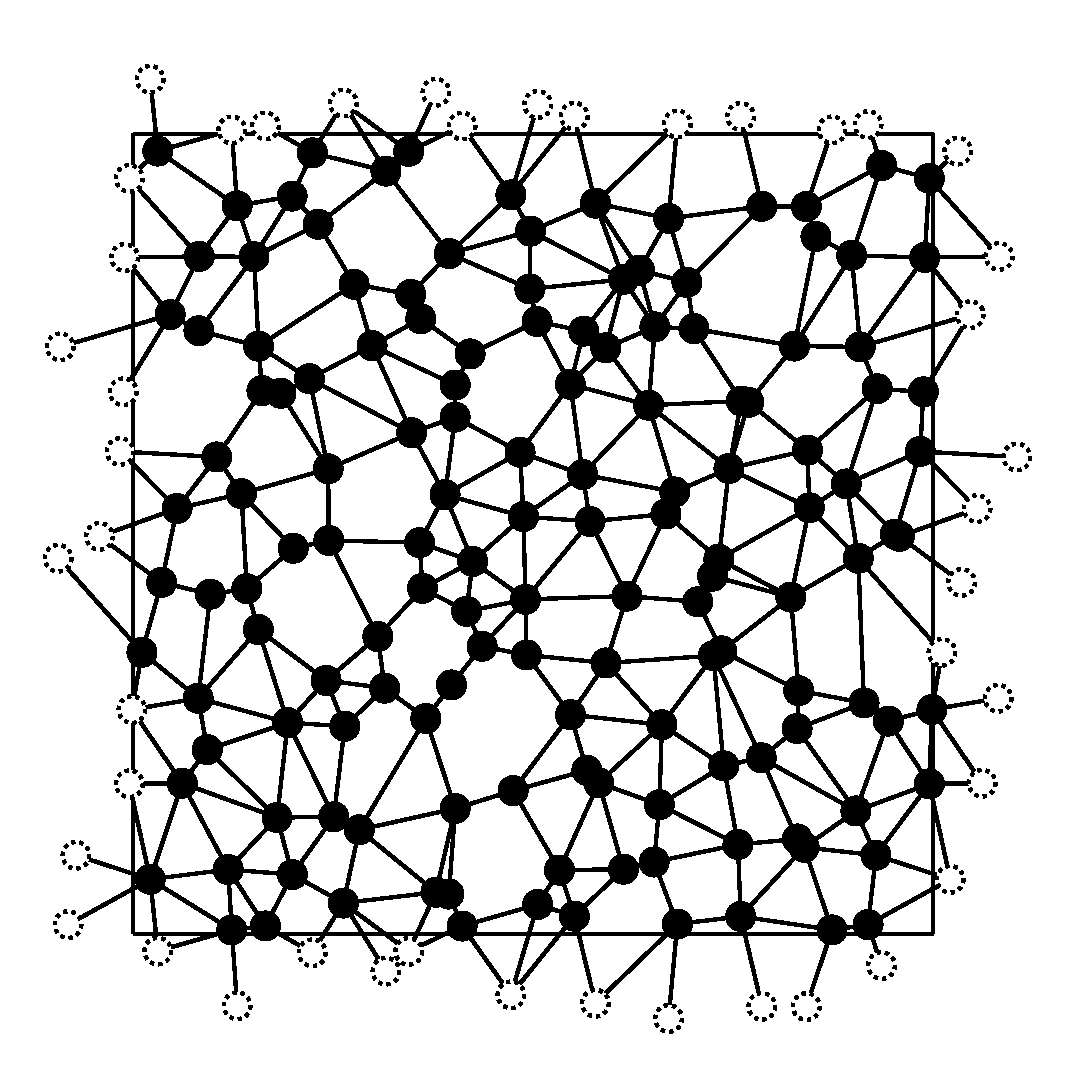
\includegraphics[width=1\textwidth]{images/GG/L12S03.pdf}
                        \caption
                        {
                            Beispiel eines GG.
                        }
                    \end{figure}
                \end{column}
            \end{columns}
        \end{frame}

        \begin{frame}{Relative Neighborhood Graph}
            \begin{columns}[b]
                \begin{column}{5cm}
                    \begin{figure}[htbp]
                        \centering
                        \begin{tikzpicture}
    \clip (-2,2.1) rectangle (2,-2);
    % Shade the intersection where signals collide.
    \begin{scope}
        \clip (-1, 0.5) circle(2.06155281281);
        \fill[fill=red!20] (1, 0) circle(2.06155281281);
    \end{scope}

    \draw (-1, 0.5) circle(2.06155281281);
    \fill (-1, 0.5) circle(0.1);
    \draw (1, 0) circle(2.06155281281);
    \fill (1, 0) circle(0.1);
    \draw (1, 0) -- (-1, 0.5);
\end{tikzpicture}

                        \caption
                        {
                            Lune eines RNG.
                        }
                    \end{figure}
                \end{column}
                \begin{column}{5cm}
                    \begin{figure}[htbp]
                        \centering
                        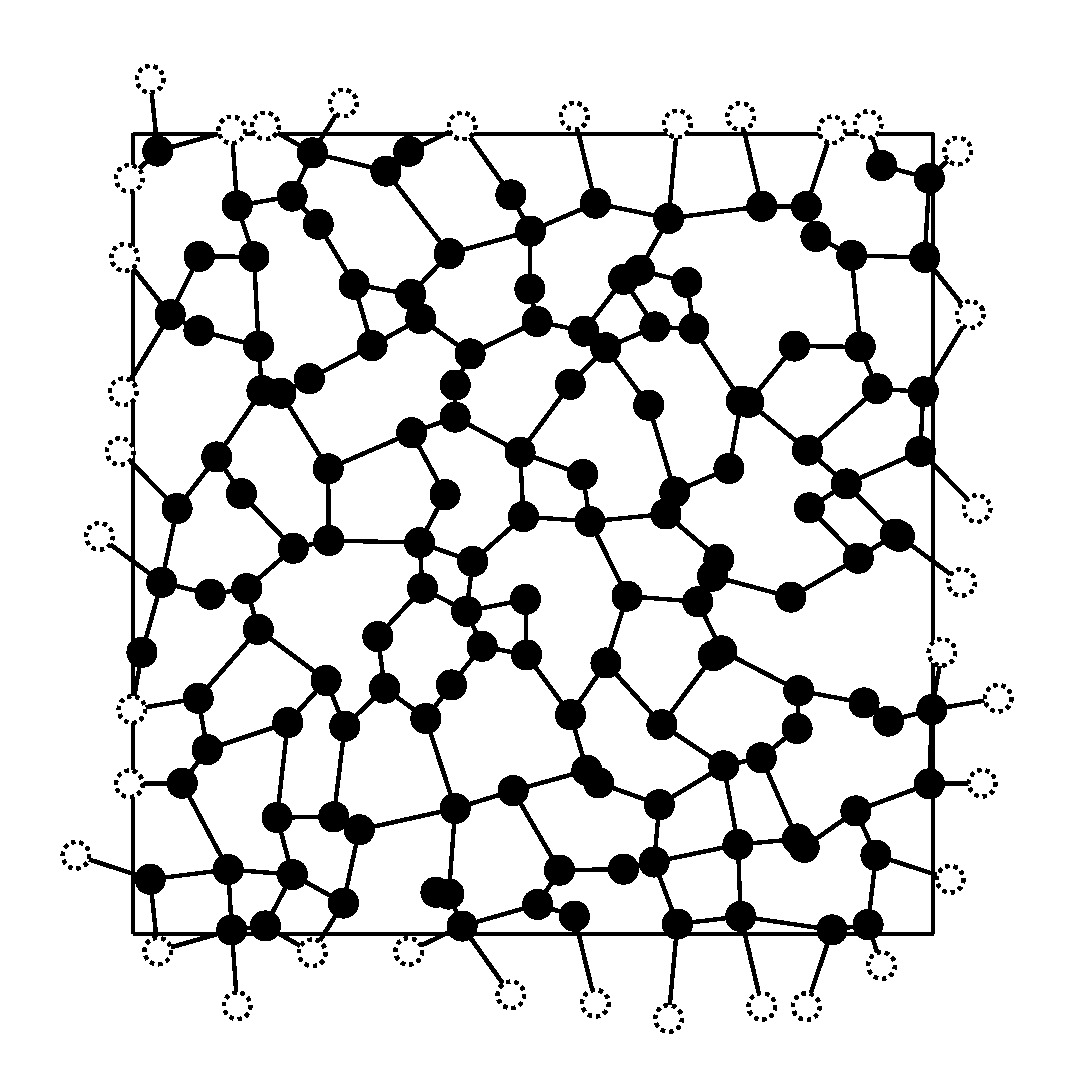
\includegraphics[width=1\textwidth]{images/RNG/L12S03.pdf}
                        \caption
                        {
                            Beispiel eines RNG.
                        }
                    \end{figure}
                \end{column}
            \end{columns}
        \end{frame}

        \begin{frame}{Graph Erzeugung}
            \begin{columns}[t]
                \begin{column}{5cm}
                    \begin{itemize}
                        \item<1-> am schnellsten: baue einen DT in \(O(n \log(n))\) und teste jede Kante
                        \item<2-> Aber DT Erstellung ist nich trivial
                        \item<3-> am einfachsten: teste jede mögliche Kante in \(O(n^{3})\)
                        \item<4-> Aber dies ist sehr langsam.
                        \item<5-> Idee: teste für jedes Paar Knoten nur Knoten nahe deren Lunes (im besten Fall \(O(n^{2})\))
                    \end{itemize}
                \end{column}
                \begin{column}{5cm}
                    \begin{overprint}
                        \onslide<6>{
                            \only<6>{
                                \begin{figure}[htbp]
                                    \centering
                                    \begin{tikzpicture}
    \foreach \x in {0,1,...,5}{
        \draw (0,\x) -- (5,\x);
        \draw (\x,0) -- (\x,5);
    }
    %random numbers generated by Python
    \foreach \x / \y in {0.28897762565/1.33479488842, 1.29507843519/0.0567389232558, 1.32094528703/3.65045643132, 2.90131976409/2.89143039453, 3.38227004393/4.97678250754, 4.78587153595/3.59043085053, 4.49289684902/0.16312339617, 2.88976245038/1.37508072608, 0.503908610931/2.15612491084, 4.29648323686/2.30979809325, 1.57506933975/4.5958939884, 3.41193951077/0.574638720997, 1.58494426782/1.67834825887, 3.87742721851/0.800878920581, 0.34861369265/2.15217676901, 3.78999774171/1.31996000053, 3.22671310651/0.945568165194, 2.58060642147/3.3521091272, 1.8091306587/0.055518765505, 4.12621981945/2.84187520295, 2.69064049175/1.18843544815, 0.248568008024/3.96126629448, 1.32959523341/3.0654517407, 4.7582022563/2.8223407318, 3.78979061396/2.79890572216}{
        \fill (\x, \y) circle(0.1);
    }
    %~ 2.58060642147/3.3521091272
    %~ 3.78999774171/1.31996000053
    \def\xa{2.58060642147}
    \def\ya{3.3521091272}
    \def\xb{3.78999774171}
    \def\yb{1.31996000053}
    \def\x{3.1853020815900002}
    \def\y{2.3360345638649997}
    \def\d{1.1823977163477497}
    \fill[blue] (\xa,\ya) circle(0.1);
    \fill[blue] (\xb,\yb) circle(0.1);
    \fill[red] (3.78979061396,2.79890572216) circle(0.1);
    \draw[blue,thick] (2,1) -- (5,1);
    \draw[blue,thick] (2,4) -- (5,4);
    \draw[blue,thick] (2,1) -- (2,4);
    \draw[blue,thick] (5,1) -- (5,4);
    \draw[blue,thick] (\x, \y) circle(\d);
\end{tikzpicture}

                                \end{figure}
                            }
                        }
                        \onslide<7>{
                                \begin{figure}[htbp]
                                    \centering
                                    \begin{tikzpicture}
    \draw[|-|] (1,5.5) -- node[above] {$L_c$} (2,5.5);
    \foreach \x in {0,1,...,5}{
        \draw (0,\x) -- (5,\x);
        \draw (\x,0) -- (\x,5);
    }
    %random numbers generated by Python
    \foreach \x / \y in {0.28897762565/1.33479488842, 1.29507843519/0.0567389232558, 1.32094528703/3.65045643132, 2.90131976409/2.89143039453, 3.38227004393/4.97678250754, 4.78587153595/3.59043085053, 4.49289684902/0.16312339617, 2.88976245038/1.37508072608, 0.503908610931/2.15612491084, 4.29648323686/2.30979809325, 1.57506933975/4.5958939884, 3.41193951077/0.574638720997, 1.58494426782/1.67834825887, 3.87742721851/0.800878920581, 0.34861369265/2.15217676901, 3.78999774171/1.31996000053, 3.22671310651/0.945568165194, 2.58060642147/3.3521091272, 1.8091306587/0.055518765505, 4.12621981945/2.84187520295, 2.69064049175/1.18843544815, 0.248568008024/3.96126629448, 1.32959523341/3.0654517407, 4.7582022563/2.8223407318, 3.78979061396/2.79890572216}{
        \fill (\x, \y) circle(0.1);
    }
    %~ 1.32094528703/3.65045643132
    %~ 1.32959523341/3.0654517407
    \def\xa{1.32094528703}
    \def\ya{3.65045643132}
    \def\xb{1.32959523341}
    \def\yb{3.0654517407}
    \def\x{1.3252702602199999}
    \def\y{3.3579540860099999}
    \def\d{0.29253431833708793}
    \fill[red] (\xa,\ya) circle(0.1);
    \fill[red] (\xb,\yb) circle(0.1);
    \draw[red,very thick] (1,3) -- (2,3);
    \draw[red,very thick] (1,4) -- (2,4);
    \draw[red,very thick] (1,3) -- (1,4);
    \draw[red,very thick] (2,3) -- (2,4);
    \draw[red,thick] (\x, \y) circle(\d);
    \draw[red,thick] (\xa, \ya) -- (\xb, \yb) ;
\end{tikzpicture}

                                \end{figure}
                        }
                    \end{overprint}
                \end{column}
            \end{columns}
        \end{frame}

\section{Methoden}
    \subsection{Monte Carlo Simulationen}
        \begin{frame}{Monte Carlo Simulationen}
            \begin{itemize}[<+->]
                \item erzeuge zufällige Zustände
                \item messe die Observablen dieser Zustände
                \item{ schätze die Observable \(O\) als
                    \begin{equation}
                        \avg{O} = \frac{1}{Z} \sum_\nu p_\nu O_\nu
                    \end{equation}
                }
            \end{itemize}
            \begin{itemize}[<+->]
                \item Aber es gibt Zustände, die mehr beitragen als andere
                \item{ zB.\ Zustände geringer Energie in kanonischen Systemen
                    \begin{equation}
                        p_{\nu} = e^{-\frac{H_{\nu}}{k_{B}T}}
                    \end{equation}
                }
            \end{itemize}
        \end{frame}

        \begin{frame}{Importance Sampling}
            \begin{itemize}[<+->]
                \item erzeuge neue Zustände entsprechend der Verteilung \(p_{i}\)
                \item effizient möglich durch Erzeugung neuer Zustände aus vorherigen
                \item{ Stichwort: Markov Kette
                    \begin{itemize}
                        \item Ergodizität\\
                                Jeder Zustand ist ein endlicher Zeit erreichbar.
                        \item Detailed Balance\\
                                Im Gleichgewicht ist die Wahrscheinlichkeit einen Zustand zu erreichen genauso groß, wie die Wahrscheinlichkeit ihn zu verlassen.
                    \end{itemize}
                }
                \item Die Korrelation aufeinanderfolgender Zustände hat einen Einfluss auf die Fehlerbalken der Observablen\\
                    \(\to\) Beachte die Autokorrelationszeit \(\tau\)
            \end{itemize}
        \end{frame}

        \begin{frame}{Single Spin Flip Metropolis Update \cite{Metropolis1953}}
            \begin{equation}
                A(\mu \to \nu) =
                \begin{cases}
                    1                            & \Delta H \le 0 \\
                    \exp{\brac{-\beta \Delta H}} & \Delta H > 0
                \end{cases}.
            \end{equation}
        \end{frame}

        \begin{frame}{Wolff Cluster Update \cite{Wolff1989}}
            \begin{equation}
                P_{\mathrm{add}} = 1-\exp\brac{-2\beta J},
            \end{equation}
            \pause
            \vspace{-1cm}
            \begin{itemize}[<+->]
                \item sehr effizient bei \(T_{c}\)
                \item ist aber Metropolis bei hohen und geringen \(T\) unterlegen
            \end{itemize}
        \end{frame}

        \begin{frame}{Parallel Tempering \cite{ParallelTempering1986}}
            \begin{equation}
                P_{\nu,\nu+1}(S_\nu \leftrightarrow S_{\nu+1}) = \min\brac{1,\exp\brac{\brac{E_{\nu+1}-E_\nu}\brac{\frac{1}{T_{\nu+1}}-\frac{1}{T_\nu}}}},
            \end{equation}
            \begin{columns}[b]
                \begin{column}{5cm}
                    \begin{figure}[htbp]
                        \centering
                        \begin{tikzpicture}
    \node[draw,rectangle] (a) {$S_1$};
    \node[draw,rectangle,right of=a] (b) {$S_2$};
    \node[draw,rectangle,right of=b] (c) {$S_3$};
    \node[rectangle,right of=c] (d) {...};

    \node[rectangle,below left of=a] (A) {};
    \node[rectangle,below right of=d] (D) {};
    \draw[thick,->] (A) edge node[below] {$T$} (D);

    \draw[thick,<->] (a) edge[out=75,in=105] node[above] {$P_{1,2}$} (b);
    \draw[thick,<->] (b) edge[out=75,in=105] node[above] {$P_{2,3}$} (c);
    %~ \draw[thick,<->] (c) edge[out=80,in=100] node[above] {$P_{..}$} (d);
\end{tikzpicture}

                        \caption
                        {
                            Austausch der Spin Konfigurationen.
                        }
                    \end{figure}
                \end{column}
                \pause
                \begin{column}{6cm}
                    \begin{figure}[htbp]
                        \centering
                        \documentclass{standalone}
\usepackage{tikz}

\begin{document}
    \begin{tikzpicture}
        %~ \draw[thick,->] (0,0) -- node[below] {$T$} (6,0);
        \draw[thick,->] (0,0) -- node[left] {$E$} (0,4);

        \draw plot [smooth] coordinates {(0,1.6) (0.2,1) (1,3.5) (1.5,0.5) (2,1.5) (2.6,3.8) (3.2,2) (3.9,2.9)};

        \fill (3.3,2.2) circle(0.1);
        \draw (1.6,0.7) circle(0.1);

        \draw[thick,|-|] (4.2,2) -- node[right] {$\Delta E$} (4.2,3.8);
        \draw[dashed] (4.2,2) -- (3.2,2);
        \draw[dashed] (4.2,3.8) -- (2.6,3.8);
    \end{tikzpicture}
\end{document}

                        \caption
                        {
                            Skizze einer Energielandschaft.
                        }
                    \end{figure}
                \end{column}
            \end{columns}
        \end{frame}

\section{Ergebnis}
    \begin{frame}{Details}
        \begin{itemize}[<+->]
            \item Ziel: Bestimme die Abhängigkeit von \(T_{c}\) und \(\sigma\)
            \item \(10^{4} (L\in\{16,32\})\) bzw.<\ \(5\cdot 10^{3} (L\in\{64,128\})\) unkorrelierte Messungen von \(O\) für \(\avg{O}\)
            \item auf jedem von 100 zufälligen proximity Graphs für \(\overline{\avg{O}}\)
            \item Messgrößen:
            \begin{itemize}[<+->]
                \item \(m = \frac{1}{N} \sum_{i} s_{i}\)
                \item \(E = \frac{1}{N} H\)
            \end{itemize}
        \end{itemize}
    \end{frame}

    \begin{frame}{Finite Size Effects}
        \begin{columns}[t]
            \begin{column}{5cm}
                \begin{itemize}[<+->]
                    \item \(T_{c}\) ist nur für \(L \to \infty\) definiert
                    \item Verschiedene Wege, um \(T_{c}\) zu bestimmen
                    \begin{enumerate}[<+->]
                        \item Finite Size Scaling lässt die Daten auf eine Kurve kollabieren
                        \begin{itemize}[<+->]
                            \item liefert auch kritische Exponenten
                        \end{itemize}
                        \item Schnittpunkte der Binder Kumulante \(g\)
                        \begin{itemize}[<+->]
                            \item sehr einfach und leicht zu automatisieren
                        \end{itemize}
                    \end{enumerate}
                \end{itemize}
            \end{column}
            \begin{column}{6cm}
                \begin{figure}[htbp]
                    \centering
                    \includegraphics[width=1\textwidth]{plots/meanM}
                    \caption
                    {
                        Finite Size Effects
                    }
                \end{figure}
            \end{column}
        \end{columns}
    \end{frame}

    \subsection{Finite Size Scaling}
        \begin{frame}{Finite Size Scaling}
            Skalen Functionen
            \begin{align}
                \label{eq:fsscaling:m}
                \avg{m_L} &= L^{-\frac{\beta}{\nu}} \tilde{M}\brac{L^\frac{1}{\nu}\brac{T-T_c}}\\
                \label{eq:fsscaling:chi}
                \chi_L    = L^{2} \beta \avg{\brac{m_{L}-\avg{m_{L}}}^2} &= L^{\frac{\gamma}{\nu}} \tilde{C}\brac{L^\frac{1}{\nu}\brac{T-T_c}}\\
                \label{eq:fsscaling:g}
                g         = \frac{3}{2}\brac{1-\frac{\avg{m_{L}^4}}{3\avg{m_{L}^2}^2}} &\propto \tilde{G}\brac{L^\frac{1}{\nu}\brac{T-T_c}}
            \end{align}
            \pause
            Durchführung mittels \texttt{autoscale.py} \cite{autoscale2009}
        \end{frame}
        \begin{frame}{Finite Size Scaling}
            \begin{figure}[htbp]
                \centering
                \subfigure
                {
                    \label{sfig:gettingCrit:binder_s_0}
                    \includegraphics[width=0.47\textwidth]{plots/binder_s_0}
                }
                \subfigure
                {
                    \label{sfig:gettingCrit:collapse_s_0}
                    \includegraphics[width=0.47\textwidth]{plots/collapse_s_0}
                }
                \caption
                {
                    Skalierung der Binder Kumulante bei \(\sigma = 0\)
                }
                \label{fig:gettingCrit}
            \end{figure}
        \end{frame}
        \begin{frame}{Finite Size Scaling}
            \begin{figure}[htbp]
                \centering
                \subfigure
                {
                    \label{sfig:gettingCrit:s_1_sus}
                    \includegraphics[width=0.47\textwidth]{plots/s_1_sus}
                }
                \subfigure
                {
                    \label{sfig:gettingCrit:collapse_s_1_sus}
                    \includegraphics[width=0.47\textwidth]{plots/collapse_s_1_sus}
                }
                \caption
                {
                    Skalierung der Suszeptibilität bei \(\sigma = 1\) auf RNG
                }
                \label{fig:gettingCrit}
            \end{figure}
        \end{frame}
        \begin{frame}{Finite Size Scaling}
            \begin{figure}[htbp]
                \centering
                \subfigure
                {
                    \label{sfig:gettingCrit:s_1_meanM}
                    \includegraphics[width=0.47\textwidth]{plots/s_1_meanM}
                }
                \subfigure
                {
                    \label{sfig:gettingCrit:collapse_s_1_meanM}
                    \includegraphics[width=0.47\textwidth]{plots/collapse_s_1_meanM}
                }
                \caption
                {
                    Skalierung der magnetisierung bei \(\sigma = 1\) auf GG
                }
                \label{fig:gettingCrit}
            \end{figure}
        \end{frame}

    \subsection{Kritische Exponenten}
        \begin{frame}{Kritische Exponenten}
            \begin{table}[htbp]
                \center
                \resizebox{\textwidth}{!}{
                    \begin{tabular}{l l l l l l}
                        \toprule
                         & \multicolumn{1}{c}{\(\sigma\)} & \multicolumn{1}{c}{\(T_c\)} & \multicolumn{1}{c}{\(\nu\)} & \multicolumn{1}{c}{\(\gamma\)} & \multicolumn{1}{c}{\(\beta\)}\\
                        \midrule
                        exakt (\cite[p. 59]{Pelissetto2002}) & \multicolumn{1}{c}{\(0\)} & 2.2691... & \multicolumn{1}{c}{\(1\)} & \multicolumn{1}{c}{\(\frac{7}{4}\)} & \multicolumn{1}{c}{\(\frac{1}{8}\)}\\
                        \midrule
                        RNG          & 0.0 & 2.2689(7)& 0.992(11)& 1.740(2) & 0.130(1) \\
                                     & 0.1 & 2.2058(8)& 0.987(12)& 1.746(5) & 0.133(4) \\
                                     & 0.2 & 1.627(2) & 1.010(9) & 1.756(14)& 0.123(10)\\
                                     & 0.5 & 1.2825(7)& 1.010(16)& 1.750(16)& 0.143(13)\\
                                     & 1.0 & 1.2123(3)& 1.013(6) & 1.758(16)& 0.138(13)\\
                        \midrule
                        GG           & 0.0 & 2.2687(5)& 0.998(8) & 1.735(2) & 0.1262(4)\\
                                     & 0.1 & 2.895(4) & 0.999(19)& 1.744(5) & 0.133(6) \\
                                     & 0.3 & 2.527(1) & 1.029(30)& 1.724(16)& 0.129(12)\\
                                     & 0.5 & 2.238(1) & 1.006(5) & 1.750(12)& 0.125(13)\\
                                     & 1.0 & 2.128(2) & 1.038(32)& 1.743(17)& 0.123(16)\\

                        \bottomrule
                    \end{tabular}
                }
                \caption
                {
                    Kritische Exponenten bei verschiedenen \(\sigma\)
                }
                \label{tab:critExp}
            \end{table}
        \end{frame}

    \subsection{Kritische Temperatur}
        \begin{frame}{Schnittpunkte der Binder Kumulante}
            \begin{columns}[t]
                \begin{column}{5cm}
                    \begin{itemize}[<+->]
                        \item Interpoliere \(g\), um die Schnittpunkte zu schätzen
                        \item Cubic Spline ist robust
                        \begin{itemize}[<+->]
                            \item stückweises Anpassen von Polynomen dritten Grades
                            \item verbinden, sodass die Kurve zweimal stetig differentierbar ist
                        \end{itemize}
                        \item Schnittpunkte sind bei \(T_{c}\) \cite{Binder1981}
                        \item einfach umzusetzten mit zB.\ \texttt{scipy}
                    \end{itemize}
                \end{column}
                \begin{column}{6cm}
                    \begin{figure}[htbp]
                        \centering
                        \includegraphics[width=\textwidth]{plots/binder_fit_s_0}
                        \caption
                        {
                            Binder Kumulante \(g\) bei \(\sigma = 0\).
                            Interpoliert mit Cubic Splines.
                        }
                        \label{fig:gettingCrit:binder_fit_s_0}
                    \end{figure}
                \end{column}
            \end{columns}
        \end{frame}

        \begin{frame}{Critical Temperature}
            \begin{figure}[htbp]
                \centering
                \subfigure
                {
                    \label{sfig:Tc:RNG}
                    \includegraphics[width=0.45\textwidth]{plots/RNG_Tc}
                }
                \subfigure
                {
                    \label{sfig:Tc:GG}
                    \includegraphics[width=0.45\textwidth]{plots/GG_Tc}
                }
                \caption
                {
                    \(T_c\) über \(\sigma\) auf RNG und GG.
                }
                \label{fig:Tc}
            \end{figure}
            \pause
            \(T_{c,RNG} \le T_{c,GG}\) während \(RNG \subseteq GG\)\\
            (vergleiche Containment Theorem für Percolation)
        \end{frame}

        \begin{frame}{Warum springt \(T_c\) auf dem GG?}
            \begin{figure}[htbp]
                \centering
                \subfigure{
                    \label{sfig:GGEdge:before}
                    \resizebox{0.43\textwidth}{!}{
                        \documentclass{standalone}
\usepackage{tikz}

\begin{document}
    \begin{tikzpicture}
        \useasboundingbox (-0.9,-0.9) rectangle (4.8,4.8);
        \draw[thick] (0,0) -- (0,4);
        \draw[thick] (0,0) -- (4,0);
        \draw[thick] (4,4) -- (4,0);
        \draw[thick] (4,4) -- (0,4);
        \fill (0,0) circle(0.2);
        \fill (4,0) circle(0.2);
        \fill (0,4) circle(0.2);
        \fill (4,4) circle(0.2);
        \draw (2,2) circle(2.82842712475);
    \end{tikzpicture}
\end{document}

                    }
                }
                \subfigure{
                    \label{sfig:GGEdge:after}
                    \resizebox{0.43\textwidth}{!}{
                        \begin{tikzpicture}
    \useasboundingbox (-0.9,-0.9) rectangle (4.8,4.8);
    \draw[dashed] (0,0) -- (0,4);
    \draw[dashed] (0,0) -- (4,0);
    \draw[dashed] (4,4) -- (4,0);
    \draw[dashed] (4,4) -- (0,4);
    \draw[thick] (0.4,0.4) -- (0,4);
    \draw[thick] (0.4,0.4) -- (4,0);
    \draw[thick] (4,4) -- (4,0);
    \draw[thick] (4,4) -- (0,4);
    \draw[thick] (4,4) -- (0.4,0.4);
    \draw[->, thick] (0,0) -- (0.2,0.2);
    \fill (0.4,0.4) circle(0.2);
    \fill (4,0) circle(0.2);
    \fill (0,4) circle(0.2);
    \fill (4,4) circle(0.2);
    \draw (2.2,2.2) circle(2.54558441227);
\end{tikzpicture}

                    }
                }
                \caption
                {
                    Kleiner GG bei \(\sigma = 0\) and \(\sigma > 0\).
                }
                \label{fig:GGEdge}
            \end{figure}
        \end{frame}

        \begin{frame}{Einfluss des Grades \(K\) auf \(T_{c}\)}
            \begin{equation}
                K = \frac{1}{N} \sum_{\avg{i,j}} 1
                \label{eq:degree}
            \end{equation}
            \begin{figure}[htbp]
                \centering
                \subfigure
                {
                    \label{sfig:deg:RNG}
                    \includegraphics[width=0.45\textwidth]{plots/RNG_deg}
                }
                \subfigure
                {
                    \label{sfig:deg:GG}
                    \includegraphics[width=0.45\textwidth]{plots/GG_deg}
                }
                \caption
                {
                    \(K\) über verschiedene \(\sigma\) auf RNG und GG.
                }
                \label{fig:Tc_deg}
            \end{figure}
        \end{frame}

\section{Überblick}
    \begin{frame}{Zusammenfassung}
        \begin{itemize}[<+->]
            \item Ungeordneter Ising Ferromagnet ist in der Universalitäts Klasse des Quadratgitter Ising Ferromagnets.
            \item Verlauf von \(T_{c}\) über \(\sigma\) ist qualitativ ähnlich zu \(K\) über \(\sigma\).
        \end{itemize}
    \end{frame}

\section{Literatur}
    \begin{frame}[allowframebreaks]
        \bibliography{lit}
        \bibliographystyle{amsplain}
    \end{frame}

\end{document}
